\documentclass[tikz, border= 10pt]{standalone}
\usepackage{pgfplots}
\pgfplotsset{compat = 1.18, width = 10cm}
\usetikzlibrary{shapes.misc}
\usetikzlibrary{patterns}
\usetikzlibrary{positioning}
\usepgfplotslibrary{fillbetween, groupplots}

\tikzset{cross/.style={cross out, draw=black, minimum size=2*(#1-\pgflinewidth), inner sep=0pt, outer sep=0pt},
%default radius will be 1pt. 
cross/.default={5pt}}

\begin{document}


%number of students chart
    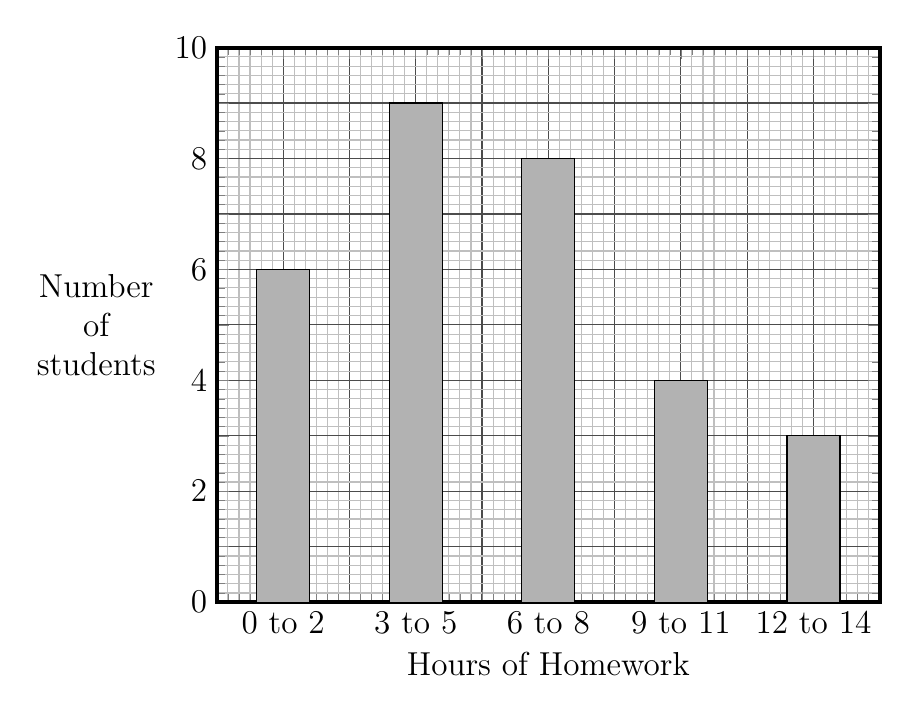
\begin{tikzpicture}
        \begin{axis}[
        title = ,
        bar width = 0.8,
        axis line style = {line width = 1.5pt, shorten >=-5mm },
        xlabel = \large Hours of Homework,
        ylabel = Number \\of \\ students,
        ylabel style = {font = \large , rotate = -90, align = center},
        ymajorgrids=true,
        xmajorgrids = true,
        xminorgrids = true,
        yminorgrids = true,
        minor grid style = {gray!50},
        minor tick num=5,
        grid style={black!70},
        xtick={0,1,2,3,4,...,10},
        xticklabels = { {}, {0 to 2}, {}, {3 to 5}, {}, {6 to 8}, {}, {9 to 11}, {}, {12 to 14}},
        xmin = 0,
        xmax = 10,
        xticklabel style = {font = \large},
        ymin = 0,
        ymax = 10,
        ytick={0,1,2,...,10},
        yticklabels = {0, {}, {2}, {}, {4}, {}, {6}, {}, {8}, {}, {10}},
        yticklabel style = {font = \large},
        clip = false,
        nodes near coords = {},
        ]
            \addplot+ [black, fill =black!30,
            ybar,
            mark = none,
            ] coordinates {
            (1,6) (3,9) (5,8) (7,4) (9,3)
            };
        \end{axis}
    \end{tikzpicture}


%number of miles chart
    \pgfplotsset{
    calculate offset/.code={
        \pgfkeys{/pgf/fpu=true,/pgf/fpu/output format=fixed}
        \pgfmathsetmacro\testmacro{(\pgfplotspointmeta *10^\pgfplots@data@scale@trafo@EXPONENT@y)*\pgfplots@y@veclength)}
        \pgfkeys{/pgf/fpu=false}
    },
    every node near coord/.style={
        /pgfplots/calculate offset,
        yshift=-\testmacro
    },
}
\pgfplotstableread{
0 3 6  
1 5 4
2 6 6   
3 7 0   
4 4 8   
}\dataset
\begin{tikzpicture}
\begin{axis}[ybar,
        bar width = 0.3,
        width=0.9\textwidth,
        ymin=0,
        ymax=8.5,        
        ylabel={Number\\ of miles},
        ylabel style = {align = center, rotate = -90},
        xtick=data,
        xticklabels = {
            Monday,
            Tuesday,
            Wednesday,
            Thursday,
            Friday
        },
        major x tick style = {opacity=1},
        minor x tick num = 1,
        minor tick length=2ex,
        ymajorgrids = true,
        legend style={at={(1.05,0.5)},anchor=west}
        ]
\addplot[draw=black,pattern=horizontal lines] table[x index=0,y index=1] \dataset; %Data1
\addplot[draw=black,pattern=north east lines] table[x index=0,y index=2] \dataset; %Data2

\legend{Paula,Rose}
\end{axis}
 \end{tikzpicture}

 
%scatter plot
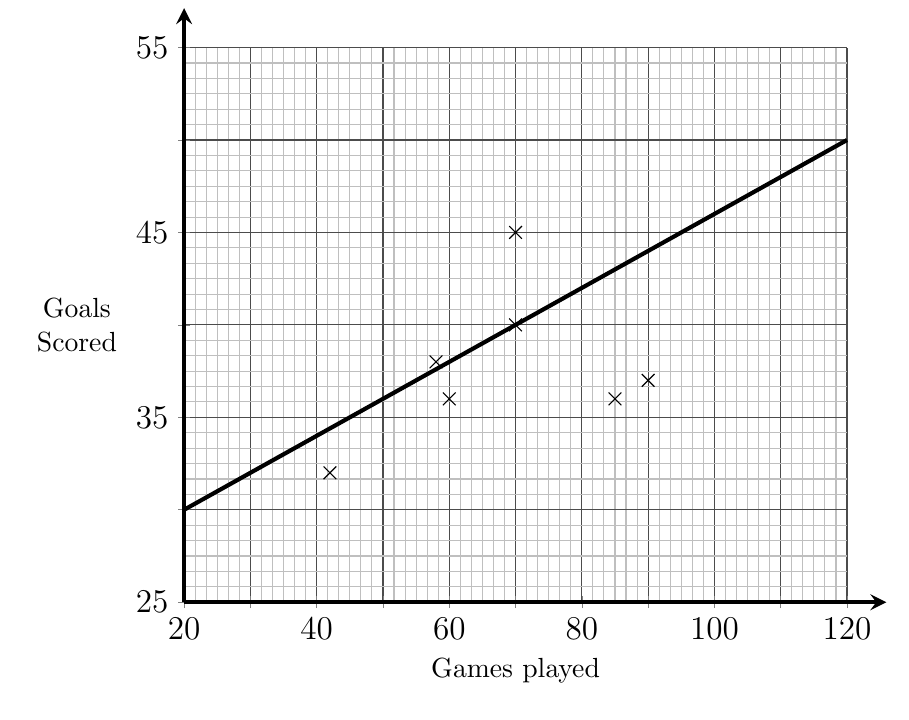
\begin{tikzpicture}
\begin{axis}
[
axis lines=left,
axis line style = {line width = 1.5pt, shorten >=-5mm},
xlabel = Games played,
ylabel = Goals \\ Scored,
ylabel style = {align = center, rotate = -90},
ymajorgrids=true,
xmajorgrids=true,
xminorgrids = true,
yminorgrids = true,
minor tick num=5,
minor tick style={draw=none},
major grid style={black!70},
minor grid style ={gray!50},
xmin=20,
xmax=120,
ymin=25,
ymax=55,
xtick={20,30,40,...,120},
xticklabels = {20, {}, 40, {}, 60, {}, 80, {}, 100, {}, 120},
xticklabel style = {font = \large},
ytick={25,30, 35,...,55},
yticklabels = {25, {}, 35, {}, 45, {}, 55},
yticklabel style = {font = \large},
tick label style={/pgf/number format/assume math mode=true},
clip = false
]

%Scatter points
\node[cross,rotate = 90,scale=0.5] at (axis cs:42,32){};
\node[cross,rotate = 90,scale=0.5] at (axis cs:60,36){};
\node[cross,rotate = 90,scale=0.5] at (axis cs:58,38){};
\node[cross,rotate = 90,scale=0.5] at (axis cs:70,45){};
\node[cross,rotate = 90,scale=0.5] at (axis cs:70,40){};
\node[cross,rotate = 90,scale=0.5] at (axis cs:85,36){};
\node[cross,rotate = 90,scale=0.5] at (axis cs:90,37){};
\addplot[color =black,line width = 1.5pt, domain = 20:120]{0.2*x + 26}; %best fit line
    \end{axis}
\end{tikzpicture}

%straight line graph
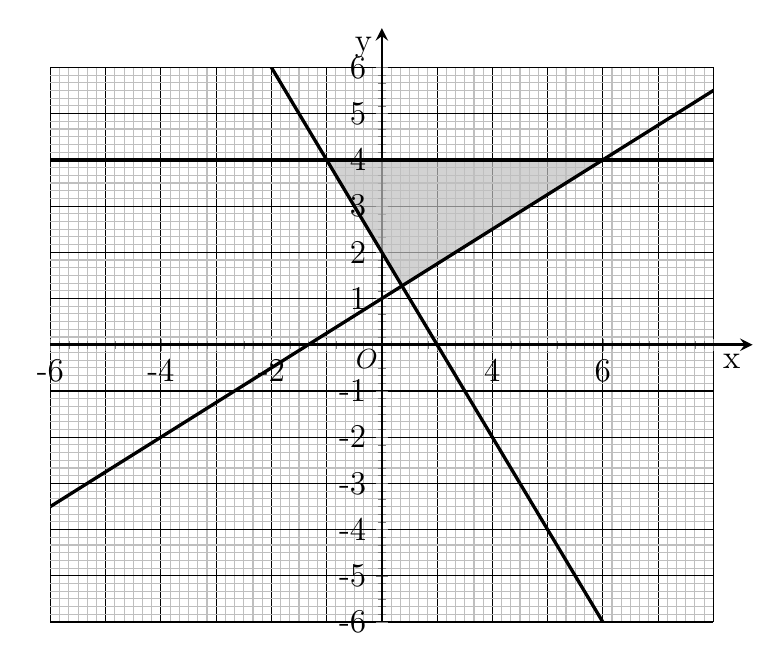
\begin{tikzpicture}
\begin{axis}
[
axis lines=middle,
axis line style = {line width = 1pt, shorten >=-5mm },
xlabel = x,
ylabel = y,
xlabel style = {anchor = north west, font = \large},
ylabel style = {anchor = south east, font = \large},
ymajorgrids=true,
xmajorgrids=true,
xminorgrids = true,
yminorgrids = true,
minor tick num=5,
minor grid style = {gray!50},
grid style={black!100},
xmin=-6,
xmax=6,
ymin=-6,
ymax=6,
xtick={-6,-5,...,6},
xticklabels = {-6, {}, -4, {}, -2, {}, {2}, {} ,{4}, {}, {6} },
xticklabel style = {font = \large},
ytick={-6,-5,...,6},
yticklabel style = {font = \large},
tick label style={/pgf/number format/assume math mode=true},
]
\node[anchor = north east] at (axis cs: 0.1,0.1) {$O$};
\addplot[color =black,line width = 1.2pt, domain = -10:10, name path = A]{0.75*x + 1};
\addplot[color =black,line width = 1.2pt, domain = -10:10, name path = B]{-2*x + 2};
\addplot[color =black,line width = 1.2pt, domain = -10:10, name path = C]{4};
\addplot[gray!50, opacity = 0.7] fill between[of=A and C,soft clip={domain=0.4:4}];
  \addplot[gray!50, opacity = 0.7] fill between[of=C and B,soft clip={domain=-1:0.4}];

    \end{axis}
\end{tikzpicture}

%histogram

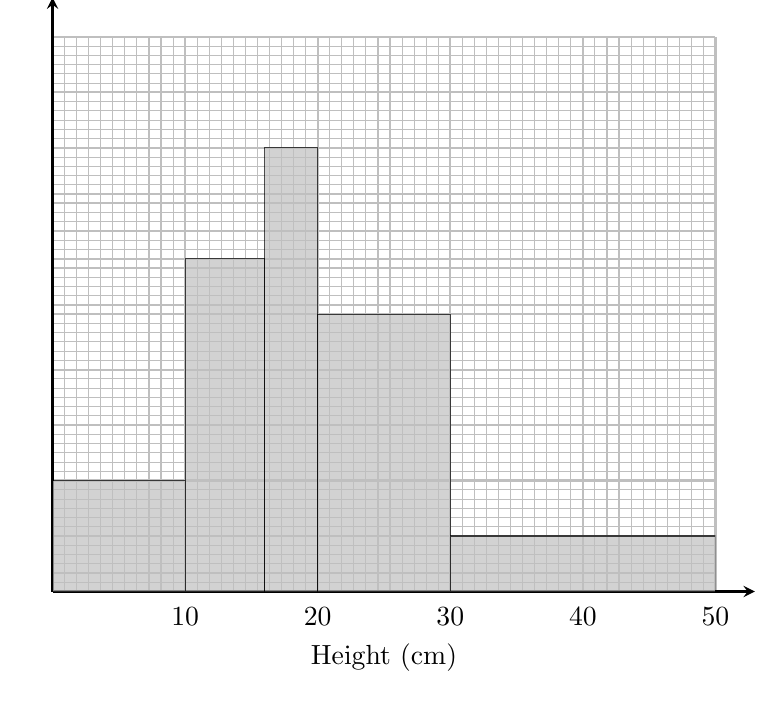
\begin{tikzpicture}
 \begin{axis}[width=10cm,
     axis lines=center,
     axis line style = {line width = 1.5pt, shorten >=-5mm},
     xmin=0,xmax=50,
     ymin=0,ymax=10,
     grid=major,
     yminorgrids,
     xminorgrids,
     ylabel near ticks,
     xlabel near ticks,
     major grid style={thick},
     tick style={thick},
     axis line style={thick},
     xlabel= Height (cm),
     ylabel=,
     xtick={0,10,...,50},
     ytick={0,1,2,...,10},
     yticklabels={},
     minor y tick num=5,
     minor x tick num=10,
     ytick style={draw=none},
     xtick style={draw=none},
     ]
    \addplot[ybar interval,fill=gray!50,draw=black, opacity = 0.7]coordinates{(0,2)(10,0)};
    \addplot[ybar interval,fill=gray!50,draw=black, opacity = 0.7]coordinates{(10,6)(16,2)};
    \addplot[ybar interval,fill=gray!50,draw=black, opacity = 0.7]coordinates{(16,8)(20,0)};
    \addplot[ybar interval,fill=gray!50,draw=black, opacity = 0.7]coordinates{(20,5)(30,0)};
    \addplot[ybar interval,fill=gray!50,draw=black, opacity = 0.7]coordinates{(30,1)(50,0)};
  \end{axis}
 \end{tikzpicture}

 %Groupplots
 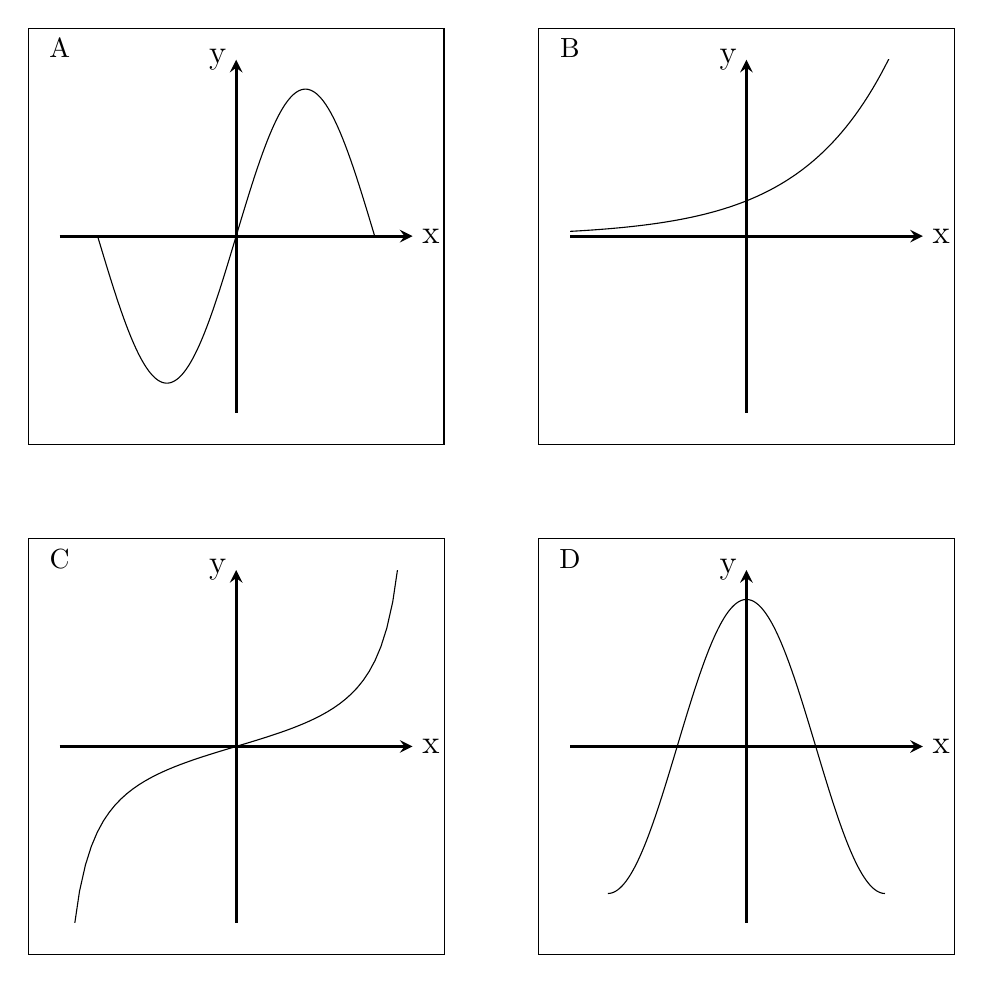
\begin{tikzpicture}
     \begin{groupplot}[group style={group name=my plots, group size= 2 by 4, horizontal sep = 2cm, vertical sep = 2cm},width=0.5\textwidth, height=0.5\textwidth,
                axis lines=middle,
                axis line style = {line width = 1pt },
                xlabel = x,
                ylabel = y,
                xlabel style = {anchor = west, font = \large},
                ylabel style = {anchor = east, font = \large},
                xmin=-4,
                xmax=4,
                ymin=-1.2,
                ymax=1.2,
                ytick style={draw=none},
                xtick style={draw=none},
                yticklabel={\empty},
                xticklabel={\empty}
                ]
        \nextgroupplot[title=]
                \addplot[domain=-pi:pi, samples = 200] {sin(deg(x))};\label{plots:plot1}
               % coordinate at top of the first plot
        \nextgroupplot[title=, ymin=-5,
                ymax=5, xmin = -2, xmax = 2]
                \addplot[samples = 200]{e^x};
        \nextgroupplot[ymax=5, ymin = -5, xmin = -1.5, xmax = 1.5]
                \addplot[samples = 200,]{tan(deg(x))};
        \nextgroupplot[title=, samples = 200]
            \addplot[ domain = -pi:pi,]{cos(deg(x))};
            
    \end{groupplot}

% Draw bounding boxes
   % Adjust the bounding box dimensions
    \foreach \i/\j in {1/1,2/1,1/2,2/2}{
        \draw ($(my plots c\i r\j.south west)+(-0.4,-0.4)$) rectangle ($(my plots c\i r\j.north east)+(0.4,0.4)$);
    }

    \node[above = -0.1cm of my plots c1r1.north west] {A};
                \node[above = -0.1cm of my plots c2r1.north west] {B};
                \node[above = -0.1cm of my plots c1r2.north west] {C};
                \node[above = -0.1cm of my plots c2r2.north west] {D};

 \end{tikzpicture}

 %Cosine function
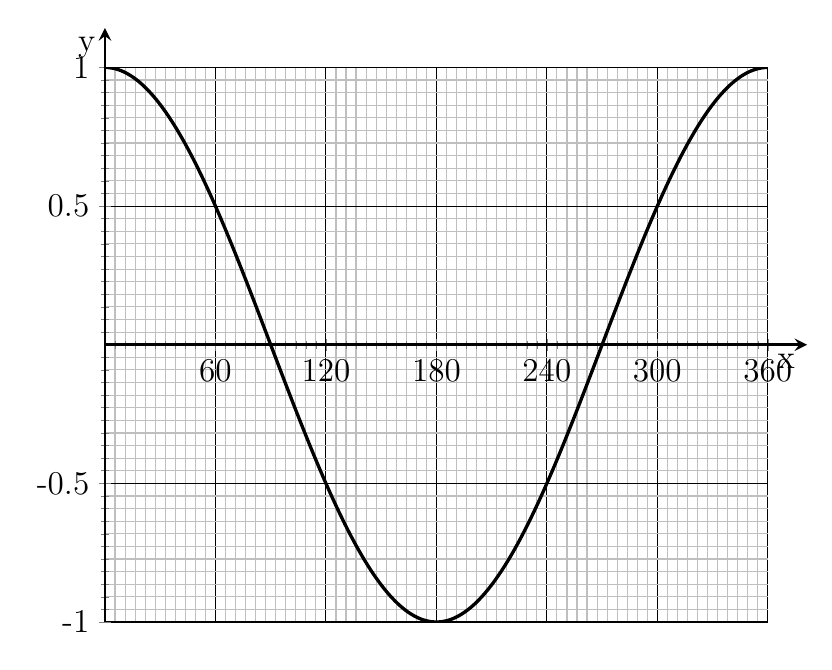
\begin{tikzpicture}
\begin{axis}[
    axis lines=middle,
    axis line style = {line width = 1pt, shorten >=-5mm},
    xlabel = x,
    ylabel = y,
    xlabel style = {anchor = north west, font = \large},
    ylabel style = {anchor = south east, font = \large},
    ymajorgrids=true,
    xmajorgrids=true,
    xminorgrids = true,
    yminorgrids = true,
    minor tick num=10,
    minor grid style = {gray!50},
    grid style={black!100},
    xmin=0,  % Set the minimum x-value to 0
    xmax=360,
    ymin=-1,
    ymax=1,
    xtick={0,60,120,...,360},  % Adjust the x-ticks for positive values only
    xticklabel style = {font = \large},
    ytick={-1,-0.5,...,1},
    yticklabel style = {font = \large},
    tick label style={/pgf/number format/assume math mode=true},
]
\node[anchor = north east] at (axis cs: -0.1,0.1) {$O$};
\addplot[color = black, samples = 200, line width = 1.2pt, domain = 0:360, name path = A]{cos(x)};

\end{axis}
\end{tikzpicture}

%cumulative curve

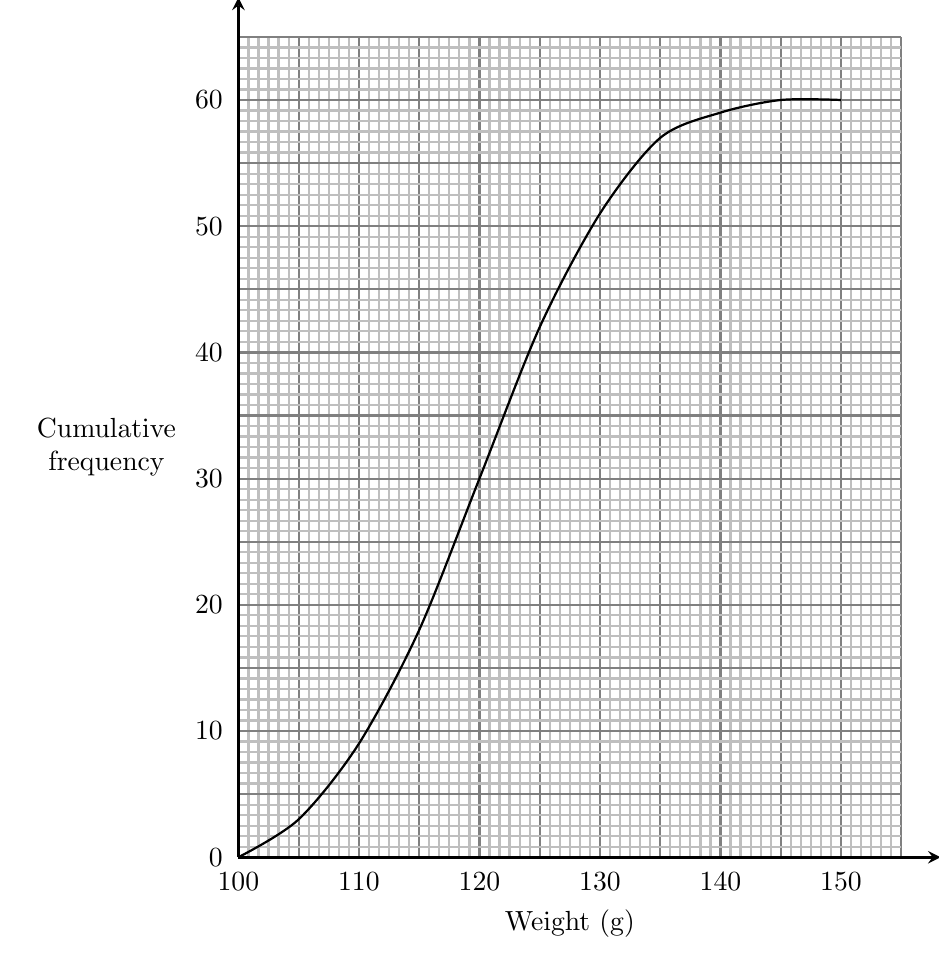
\begin{tikzpicture}
    \begin{axis}[
        title={},
        axis lines=left,
        axis line style = {line width = 1pt, shorten >=-5mm},
        width = 10cm,
        height = 12cm,
        xlabel={Weight (g)},
        ylabel={Cumulative \\ frequency},
        ylabel style = {rotate = -90, align = center},
        grid=major,
        xminorgrids = true,
        yminorgrids = true,
        minor tick num=5,
        minor grid style = {gray!50},
        grid style={gray!100, thick},
        ymin=0,
        ymax=65,
        xmax=155,
        xmin=100,
        xtick={100,105,...,155},
        xticklabels = {100, {}, 110, {}, 120, {}, 130, {} ,140, {}, 150, {} },
        ytick={0,5,...,65},
        yticklabels = {0, {}, 10, {}, 20, {}, 30, {} ,40, {}, 50, {}, 60, {} },
        ytick style={draw=none},
        xtick style={draw=none},
        enlarge x limits=false,
        enlarge y limits=false
    ]
    % The cumulative curve with more points for a smoother S-like shape
    \addplot+[smooth, no marks, thick, black] 
        coordinates {(100,0) (105,3) (110,9) (115,18) (120,30) (125,42) (130,51) (135,57) (140,59) (145,60) (150,60)};
    \end{axis}
\end{tikzpicture}

\end{document}